\documentclass[12pt]{article}

\usepackage{sbc-template}
\usepackage{amsmath}
\usepackage{graphicx,url}

\usepackage[brazil]{babel}   
%\usepackage[latin1]{inputenc}  
\usepackage[utf8]{inputenc}  
% UTF-8 encoding is recommended by ShareLaTex

\sloppy

\title{Um breve estudo sobre buscas no contexto de IA }

\author{Kim Bemfica Agliardi}


\address{Instituto de Informática -- Universidade do Vale do Rio dos Sinos
  (Unisinos)\\
  Caixa Postal 275-- 93022-000 -- São Leopoldo -- RS -- Brasil
  \email{\ kim.agliardi@edu.unisinos.br}
}

\begin{document} 

\maketitle

\section{Introdução}

Este artigo foi realizado como atividade complementar do Grau A da disciplina de inteligência artificial, tendo como objetivo, exercitar o conhecimento de sobre como os problemas são formulados e resolvidos em IA, utilizando estratégias de busca informadas e não informadas.

\section{Conceitos gerais} \label{sec:concepts}
Em IA é possível construir um conjunto de estados para encontrar uma sequência de ações cuja aplicação resolve um problema. O processo de tentar encontrar uma sequência de ações que leve de um estado até um estado objetivo é chamado de busca. 
Um problema pode ser decomposto em cinco itens, conforme a figura abaixo:

\begin{figure}[h]
    \centering
    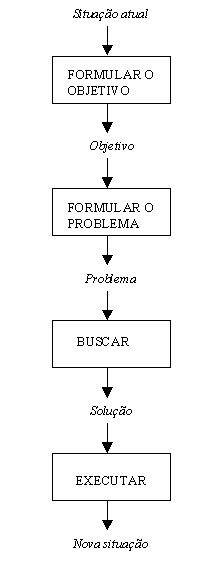
\includegraphics[scale=.6]{figura1.jpg}
    \caption{Modelagem Problema}
    \label{fig:figura1.jpg}
\end{figure}

A formulação de objetivo nada mais é do que a definição do conjunto de estados que satisfazem o objetivo.
A formulação do problema é a decisão de quais estados devem ser considerados, neste passo, também podem ser abstraídas informações que não são consideradas pertinentes à resolução do problema.
Já na etapa de busca, temos o exame de várias sequencias de ações possíveis e as estratégias de controle possíveis.

\subsection{Busca}
Ao longo desta subseção, abordaremos os principais tópicos sobre o tema de busca, tais como: buscas cegas, bucas informadas, estruturas de controle, etc..

Métodos de busca consistem:
\begin{itemize}
    \item Geração dinâmica de uma árvore, representando os estados alcançáveis a partir de um estado;
    \item A seleção do estado a ser expandido é determinado pela estratégia de controle;
    \item O processo para quando o estado designado por um nó folha corresponde ao objetivo.
\end{itemize}

Podemos definir as estruturas de controle necessários nos seguintes pontos:

\begin{itemize}
    \item \textbf{Nó}: Consiste em um estado, nó pai, operador utilizado para produzir o nó, sua profundidade e o custo total até este nó;
    \item \textbf{Fila}: Contém todos os nós produzidos que aguardam para ser expandidos. Estes nós constituem a fronteira da busca;
\end{itemize}
A avaliação da estratégia de controle consiste em:
\begin{itemize}
    \item \textbf{Completeza}: Garantia de encontrar uma solução, se existir;
    \item \textbf{Otimalidade}: Estratégia de busca encontra uma solução ótima;
    \item \textbf{Complexidade temporal}: Tempo levado para encontrar uma solução;
    \item \textbf{Complexidade espacial}: Quantidade de memória utilizado para a busca.
\end{itemize}
Ainda sobre solução de problemas: 
\begin{itemize}
    \item Uma solução para um problema é uma sequência de ações que conduzam do estado inicial para o estado objetivo;
    \item Uma solução ótima é uma solução com o menor custo de caminho.
\end{itemize}

\subsubsection{Busca cega}
Métodos de busca cega fazem uma pesquisa sistemática do espaço de estados, porém, não utilizam nenhum conhecimento para guiar esta busca. Os três principais métodos cegos são a \textbf{busca em profundidade}, \textbf{busca em largura} e a \textbf{busca com custo uniforme}. 
A ação de percorrer o espaço de estados é feita de acordo com a estratégia de controle que seleciona um estado e um operador que será aplicado ao estado para gerar os estados subsequentes. A aplicação dos operadores nos estados iniciais e intermediários é feita até que se encontre um estado objetivo. A medida que o processo é executado, é gerada a árvore de busca. Quando se chega ao estado final, o processo é interrompido com sucesso. Dependendo do problema, a solução pode ser o próprio estado final ou o caminho entre o estado inicial e o estado final.  

\subsubsection{Busca informada}
Métodos de busca informada possuem um "domínio", isto é, quando podemos fornecer informações de proximidade ao objetivo. Se sabemos onde está o estado final, podemos direcionar a busca nesta direção.
Algoritmos de busca informada, geralmente são mais rápidos e eficientes, explorando menos nós no grafo. Mas como dito anteriormente, para utilização destes algoritmos, precisamos informar a proximidade até o alvo em cada nó do grafo.

\paragraph{Heurísticas} no contexto de \textbf{busca informada} são funções que realizam uma estimativa de valor (uma distância, por exemplo) entre um estado e o estado final da busca. A diferença entre algoritmos gerais e algoritmos que utilizam buscas com heuristicas, é que o segundo, utiliza uma função que atribuir um valor a cada nó n da lista dos nós abertos (os nós que estão aguardando para ser expandidos). O nó que possui o menor valor, é o escolhido para continuar a busca.
Porém, se utilizarmos apenas heurísticas, teremos a \textbf{busca gulosa}, que sempre explora o vértice aparentemente mais próximo do objetivo.
Se somado o custo percorrido a uma estimativa de quanto falta até o objetivo, temos a busca A*.
É dito que esses algoritmos são de busca informada pois eles conhecem a localização do objetivo e podem usar esta informação para estimar quanto falta para chegar ao objetivo.
A busca gulosa é \textbf{completa} desde que o grafo pesquisado seja acíclico, ela também não é ótima e em geral, é mais rápida que a busca de custo uniforme (expande uma quantidade menor de vértices).
\paragraph{Busca A*} é identitica à busca de custo uniforme e à gulosa, porém, a ordenação da fila de prioridades é feita pela \textbf{soma} do custo percorrido com a estimativa da distância restante.
custo total = percorrido + estimado
A busca A* é completa e ótima, desde que:
\begin{itemize}
    \item A heurística usada seja textbf{admissível};
    \item Uma heurística é dita admissível se ela \textbf{não superistima o custo real};
    \item Ou seja podemos errar as estimativas para valores \textbf{menores}, mas nunca maiores;
    \item Em problemas de mapas em geral, a distância em linha resta é uma boa heurística: é impossível fazer um trajeto menor que a linha reta, portanto a estimativa nunca fica acima do valor real.
\end{itemize}
Ainda, algoritmos de busca informada não são restritos a grafos de mapas. Assim como qualquer algoritmo de busca em grafos, eles são genéricos, porém, é preciso definir heurísticas adequadas para cada tipo de problema.


\section{Situação analisada}

Para execução deste trabalho, utilizei como base uma implementação em Python, que foca na resolução do problema que consiste na movimentação de um personagem dentro de um labirinto com obstáculos. 
Os seguintes estados são possíveis no arquivo CSV que compõe a matriz deste labirinto:
\begin{itemize}
    \item \textbf{0} - Representa a saída do labirinto;
    \item \textbf{1} - Representa um caminho livre para deslocamento;
    \item \textbf{2} - Representa um obstáculo;
    \item \textbf{3} - Representa o estado inicial(posição) do personagem.
\end{itemize}
O personagem pode se deslocar ao longo do labirinto, podendo realizar movimentos para cima e para baixo e para os lados, assim como movimentos diagonais. Um exemplo de matriz possível seria:
\[
\begin{matrix}
5 & 5 \\
3 & 1 & 1 & 1 & 1 \\
1 & 2 & 1 & 1 & 1 \\
1 & 1 & 2 & 2 & 1 \\
1 & 1 & 1 & 1 & 1 \\
1 & 2 & 1 & 1 & 0 \\
\end{matrix}
\]

Aonde o primeiro elemento \textbf{5} seria o número de linhas e o segundo \textbf{5} representaria o número de colunas.
Optei por este problema por ser algo previamente abordado em sala de aula e por possuir das mais diversas implementações e exemplos pela internet,facilitando assim o meu entendimento sobre o conteúdo. Para a resolução do problema, foram aplicadas as buscas \textbf{A*}  e \textbf{BFS}, uma informada e outra não informada.

\section{Técnicas utilizadas}
Conforme informado anteriormente, foram utilizadas duas abordagens para a resolução do problema, uma envolvendo uma busca informada (que utiliza uma determinada heurística) e outra que testa os estados exaustivamente, até o encontro ou não da solução.
Falando especificamente da busca \textbf{A*}, é aplicada uma função heurística baseada na distância percorrida pelo personagem, acrescentando a distância euclidiana "g" entre a localização do nosso personagem e o seu destino. A distância "f" que já foi percorrida é de fácil cálculo, pois é apenas um acréscimo a cada movimentação. Já a distância até o ponto final, é uma estimativa do tamanho em linha reta entre os dois pontos, já que esta se trata de uma estimativa otimista (o menor caminho entre dois pontos é sempre uma reta). Sendo assim, o cálculo desta heuristica é: h = f(estado) + g(estado, meta).
O cálculo da distância euclidiana entre um Ponto1 e um Ponto2 é dado por: \begin{equation}
    g(Ponto1,Ponto2) = \sqrt{(x1-x2)^2 + (y1-y2)^2}
\end{equation}

Já a estratégia de busca do \textbf{BFS} visa realizar a expansão de cada estado que está em sua fila, por exemplo, se agora estou na posição (6,3), é possível que meus próximos passos sejam [(6, 3), (5, 3), (4, 4), (3, 4), (2, 4), (1, 4),etc..], a ideia sempre será verificar o estado que a mais tempo está na lista, e descartá-lo após a verificação em cada etapa do \textbf{BFS}. Após um estado ser expandido, os próximos serão adicionados à fila e ficam "linkados" ao estado que os gerou, permitindo que ao final da busca o caminho do estado de inicio até o estado final possa ser reconstruído.

\section{Análise das técnicas}
Para a análise das técnicas, utilizei a mesma matriz 5x5 descrita como labirinto na seção \textbf{Problema}, foi possível observar a superioridade da busca \textbf{A*}, a qual necessitou de apenas 6 iterações para atingir o estado final, já a busca \textbf{BFS} precisou realizar 21 iterações para atingir o estado final. Ambas execuções e análises estão anexas ao trabalho, optei por não inseri-lás aqui pois poluiria muito o texto.

\section{Conclusão}
As duas técnicas utilizadas fornecem uma solução para o problema, porém, geralmente, a busca \textbf{A*} oferece uma solução mais eficiente, pelo fato de obter um direcionamento e necessitar de um menor número de iterações. As duas buscas possuem um valor de iterações semelhantes apenas quando de fato não há outros caminhos possíveis de um estado inicial para um estado final.
Por fim, acredito que a pesquisa para este trabalho tenha sido de grande valia para o entendimento da matéria de buscas e de formulação de problemas e nos mostrando que diversas soluções de problemas podem ser resolvidos a partir de uma formulação de problema e da aplicação de técnicas de busca.




\section{Referencias}
\cite{Russel:09}
\bibliographystyle{sbc}
\bibliography{sbc-template}

\end{document}
